\documentclass[fleqn]{article}
\usepackage[nodisplayskipstretch]{setspace}
\usepackage{amsmath, nccmath}
\usepackage{amssymb}
\usepackage{enumitem}
\usepackage{etoolbox}
\usepackage{graphicx}

\newcommand{\zerodisplayskip}{
	\setlength{\abovedisplayskip}{0pt}%
	\setlength{\belowdisplayskip}{0pt}%
	\setlength{\abovedisplayshortskip}{0pt}%
	\setlength{\belowdisplayshortskip}{0pt}%
	\setlength{\mathindent}{0pt}}

\makeatletter
	\newenvironment{equationCenter}{\@fleqnfalse\begin{equation*}}{\end{equation*}}
\makeatother

\title{Homework 4}
\author{Owen Sowatzke}
\date{October 16, 2023}

\begin{document}
	\offinterlineskip
	\setlength{\lineskip}{12pt}
	\zerodisplayskip
	\maketitle
	
	\begin{enumerate}[nolistsep]
		\item Define $T \in \mathcal{L}(\mathbb{F}^2)$ by
		
			\begin{equationCenter}
				T(w,z) = (z,w)
			\end{equationCenter}
			
			Find all eigenvalues and eigenvectors of $T$.
	
			$Tv = {\lambda}v$
			%
			$\Rightarrow T(w,z) = \lambda(w,z)$
			%
			$\Rightarrow(z,w) = \lambda(w,z)$
			%
			$\Rightarrow(z,w) = ({\lambda}w,{\lambda}z)$
			
			$z = {\lambda}w$
			%
			$\Rightarrow w = \lambda({\lambda}w)$
			%
			$\Rightarrow w = {\lambda}^2 w$
			%
			$\Rightarrow {\lambda}^2 = 1$
			%
			$\Rightarrow \lambda = \pm \sqrt{1}$
			%
			$\Rightarrow \lambda = \pm 1$
			
			$\therefore \lambda_1 = 1,\ \lambda_2 = -1$
			
			$\lambda_1 = 1 \Rightarrow z = w \Rightarrow v_1 = (w, w)$
			
			$\lambda_2 = -1 \Rightarrow z = -w \Rightarrow v_2 = (w, -w)$
			
		\item Suppose $T \in \mathcal{L}$ and $\text{dim range}\ T = k$. Prove that $T$ has at most $k + 1$ distinct eigenvalues.
	
			Let $v_j$ be an eigenvector of $T$. Then, $Tv_j = {\lambda_j}v_j$.
			
			Consider $\lambda_j \neq 0$:
			
			\begin{equation*}
				\Rightarrow \frac{1}{\lambda_j}T(v_j) = v_j \Rightarrow T\left(\frac{v_j}{\lambda_j}\right) = v_j	 \Rightarrow v_j \in \mathcal{R}(T)			
			\end{equation*}
			
			There are at most $k$ linearly independent eigenvectors $v_j$.
			
			For $\lambda_j$ to be distinct eigenvalues, each $v_j$ must be linearly independent.
			
			$\therefore$ there can be at most $k$ distinct nonzero eigenvalues $\lambda_j$.
			
			\pagebreak
			Consider $\lambda_j = 0$:
			
			For $\lambda_j=0$, there must be a nonzero eigenvector $v_j$ s.t.
			
			$Tv_j = 0 \Rightarrow v_j \in n(T)$
			
			Let $n(T) \neq \{0\} \Rightarrow \exists\ v_j \neq 0$ s.t. $Tv_j = 0$
			
			For this case, $\exists\ \lambda_j = 0$
			
			$\therefore$ there are at most $k + 1$ distinct eigenvalues.
		
		\item \textbf{Electrical Oscillators:} Consider the electric circuit shown below.
		
			\begin{center}
				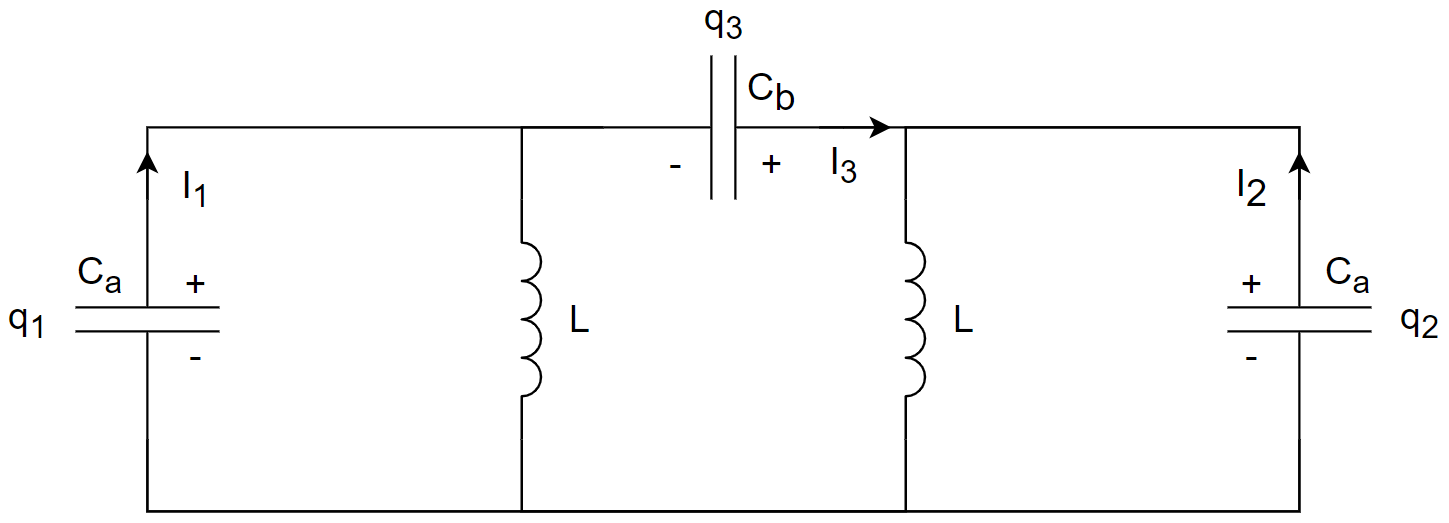
\includegraphics[width=0.75\textwidth]{Homework4_Circuit_Sowatzke.png}
			\end{center}
	\end{enumerate}
\end{document}